%% ============================================================================================================
%% Computational experiment
%% ============================================================================================================
\section{Computational experiment}
\label{sec:computational-experiment}

% Software
% ————————————————————————————————————————————————————————————————————————————
\subsection*{Software}
% \begin{refcontext}[style=numeric]
All experiments were conducted in Python 3.12 using the following open-source libraries:
\begin{itemize}
    \item \texttt{scikit-learn} (version *.*.*) for implementation of Random Forest models~\cite{pedregosaScikitlearnMachineLearning}.
    \item \texttt{XGBoost} (version *.*.*) for gradient boosting models~\cite{chenXGBoostScalableTree2016a}.
    \item \texttt{Dask} (version ) for parallel and distributed computation~\cite{rocklinDaskParallelComputation2015}.
    \item \texttt{NumPy} and \texttt{Pandas} for data manipulation and preprocessing.
    \item \texttt{Matplotlib} and \texttt{Seaborn} for visualization.
\end{itemize}
Experiments were executed on a machine \todo{describe the machine}. The complete source code and environment configuration files are available at: \url{https://github.com/intsystems/2025-Project-188}.
% \end{refcontext}

\subsection{Correlation analysis}

To eliminate model equifinality arising from mathematical similarity among features (which is especially critical for tree-based algorithms), we conducted a correlation analysis\ref{fig:corr-analysis} using Pearson’s correlation coefficient. From the full feature set, 20 static features and 3 ``reserve'' features (duplicating the main ones when some data were missing) were selected. For the final feature selection, we first computed the sum of absolute correlations of each feature with all others, chose those with the lowest totals, and then picked the most readily interpretable features from that subset.

\begin{center}
    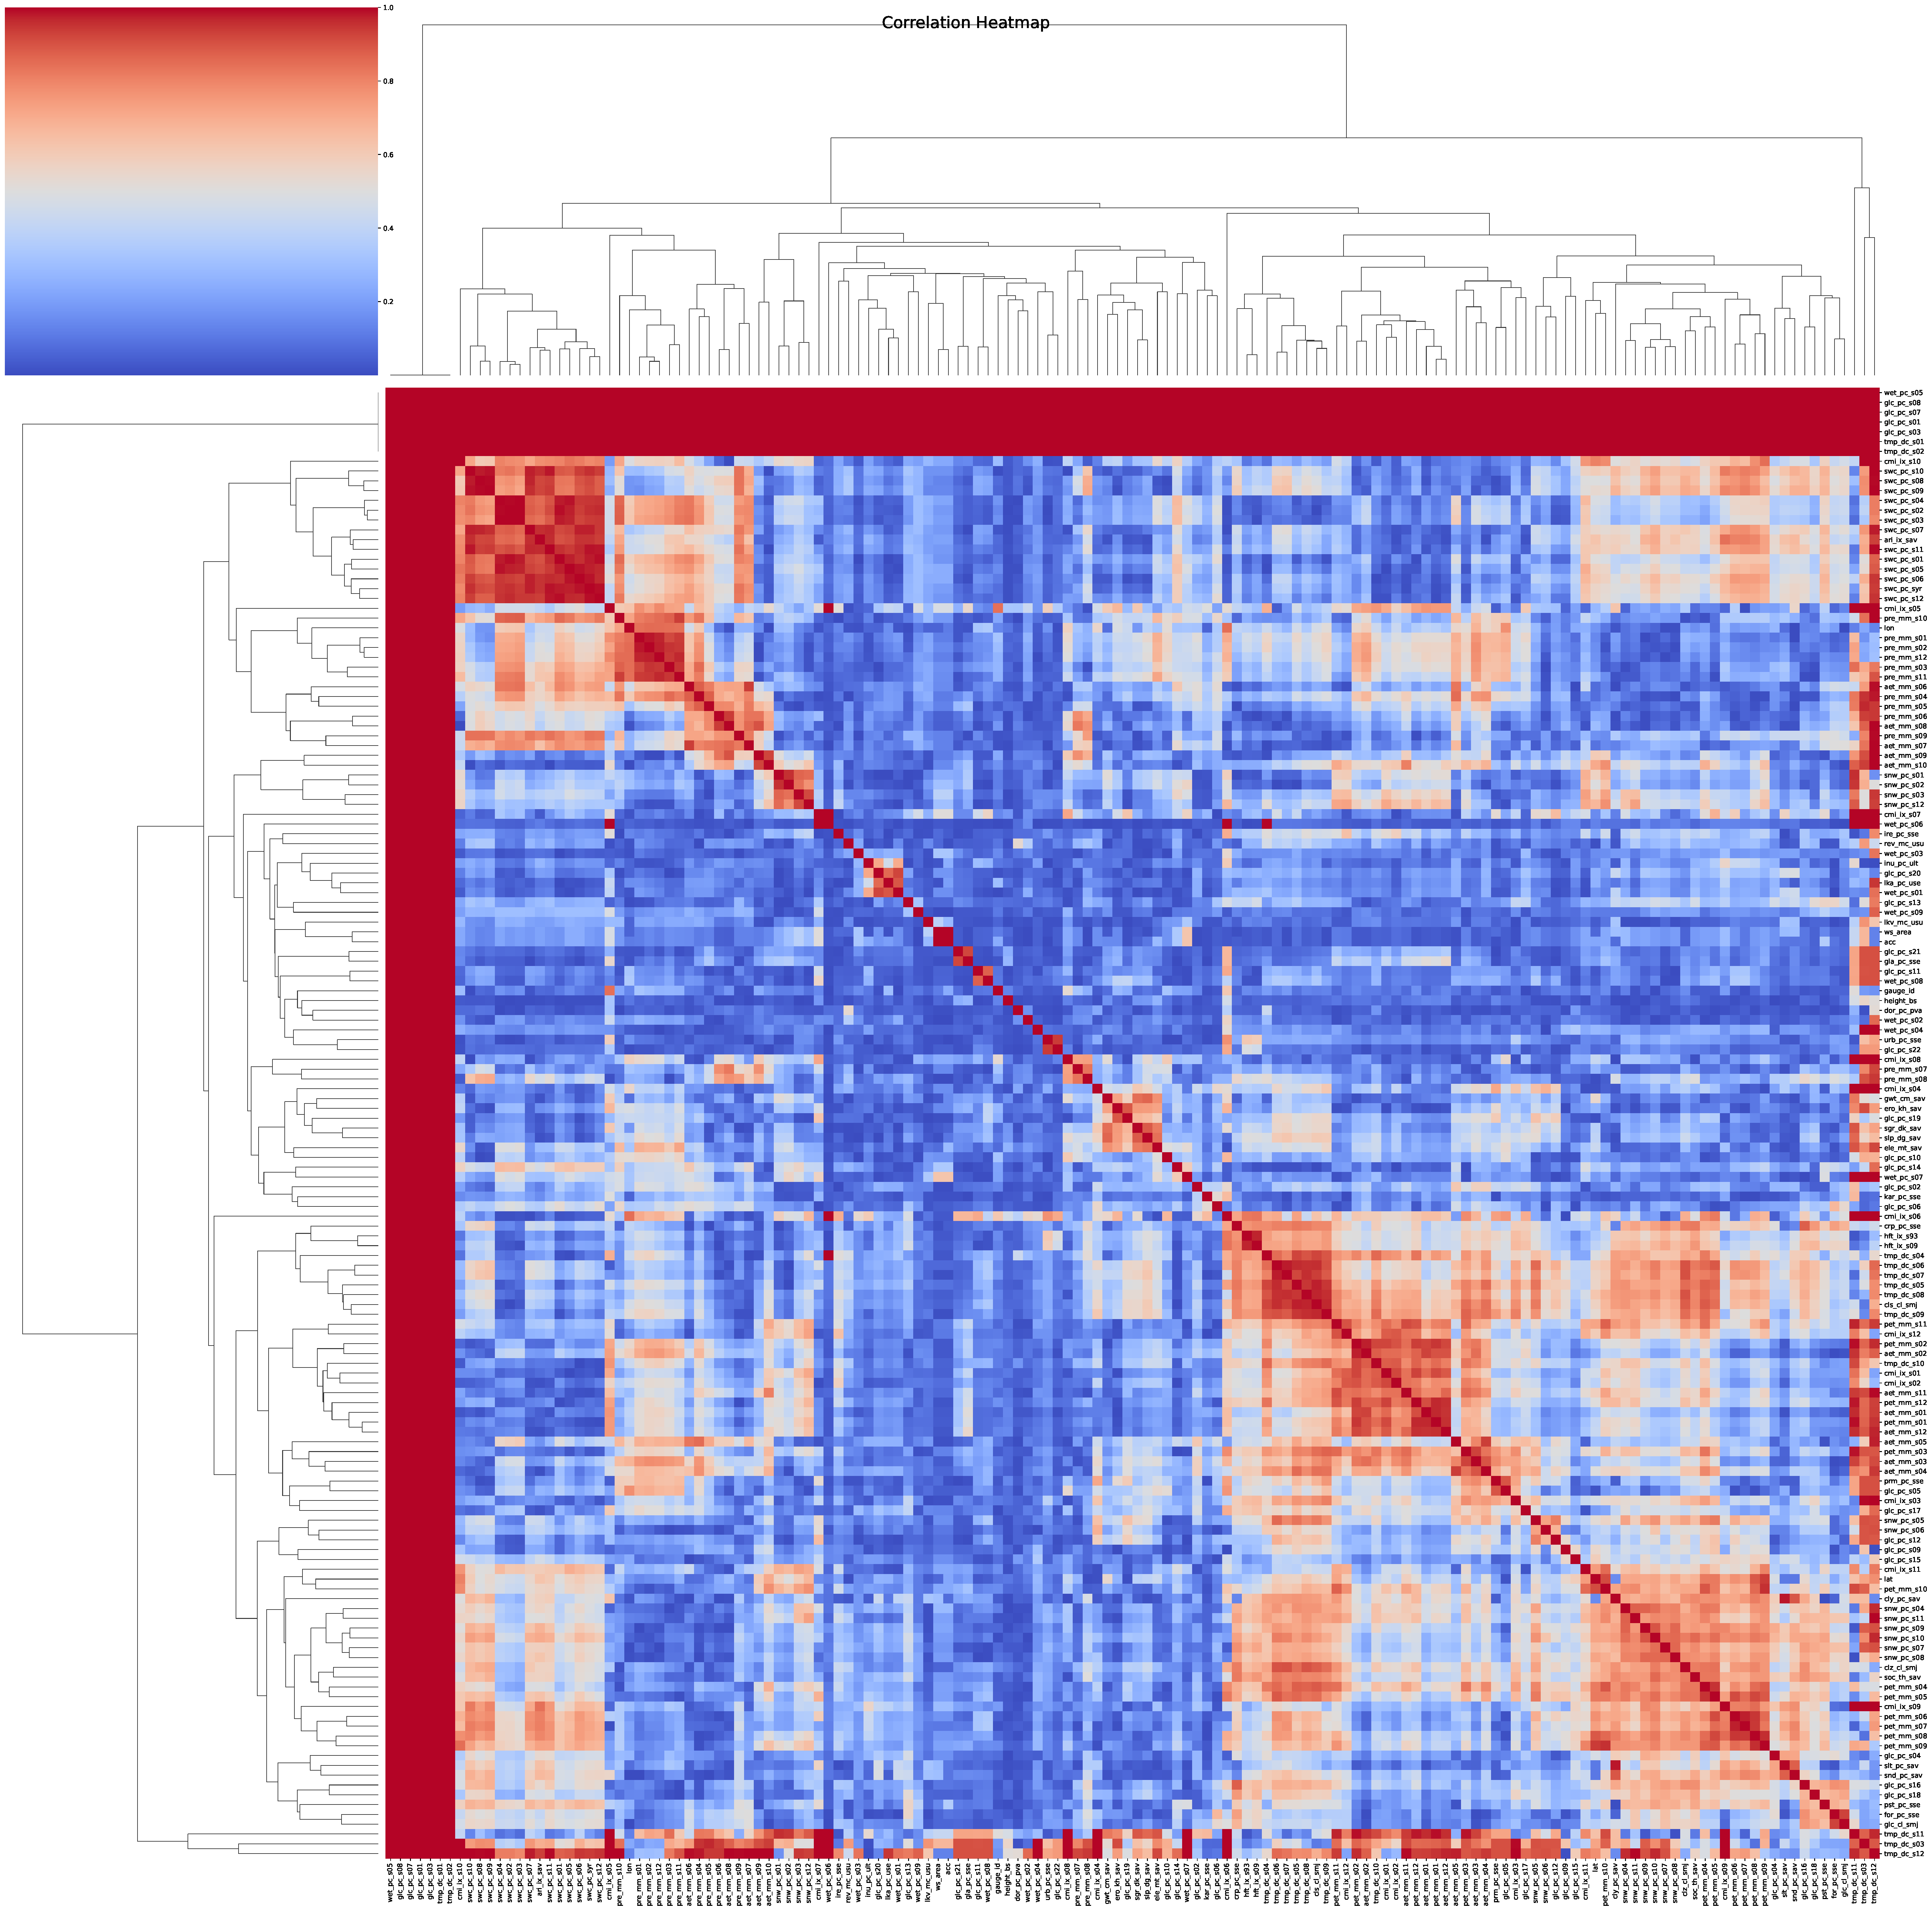
\includegraphics[width=0.6\textwidth]{bin/static_features_heatmap.pdf}
    \label{fig:corr-analysis}
\end{center}

\subsection{Clusterization}

To assess how well the models actually capture hydrological patterns, we grouped river basins into clusters based on static features. After training on the full dataset, we expected the model to assign each basin to its cluster and recognize these groups as significant. We conducted a visual analysis of clustering using the k-means algorithm with prior standard scaling of the features. The number of clusters was varied from 5 to 14, and based on the heatmap that most clearly reflected differences among basins by their static attributes, we decided to use nine clusters.


\subsection{Data-Processing Pipeline}
\begin{enumerate}
    \item Split the dataset into training (train) and validation (valid) sets;
    \item Perform hyperparameter tuning with Optuna to select the optimal model within each algorithm class;
    \item Train the model on the training set;
    \item Conduct feature-importance analysis using SHAP for each model class;
    \item Compare models based on key metrics on both the training and validation sets.
\end{enumerate}
